%% Subject template with multiple examples
%%
%% Based on Overleaf's Technical Document Template
%% https://www.overleaf.com/latex/templates/technical-document-template/mdgftpdfbvbs

\documentclass{../sujet-tp-ateliers}

% Include every required package in this page

\RequirePackage{fullpage,parskip}
\RequirePackage[utf8]{inputenc}
\RequirePackage[T1]{fontenc}
\RequirePackage[sfdefault]{roboto}
\RequirePackage[scaled=0.95]{roboto-mono}
\RequirePackage{hyperref}
\RequirePackage{xcolor}
\RequirePackage{graphicx}
\RequirePackage{microtype}
\RequirePackage{tcolorbox}
\RequirePackage{amsmath}
\RequirePackage{amssymb}
\RequirePackage{sfmath}
\RequirePackage{mathtools}
\RequirePackage{mathrsfs}
\RequirePackage{fancyhdr}

%%%%%%%%%%%%%%%%%%%%%%%%%%%%%%%%%%%%%%%%%%%
% DO NOT MODIFY ANYTHING ABOVE THIS BLOCK %
%%%%%%%%%%%%%%%%%%%%%%%%%%%%%%%%%%%%%%%%%%%

% Frontmatter data; appears on title page
\newcommand\gettitle{Arduino\\Prototypage avec Tinkercad}
\newcommand{\getversion}{0.1}
\title{\gettitle}
\version{\getversion}
\author{Malo Garnier}
\logo{
\includegraphics[width=8cm]{../../static/logo}}

\begin{document}

\maketitle

\setcounter{page}{1}

% configure header & footer
\pagestyle{fancy}
\fancyhf{} % clear all header and footer fields
\fancyhead[L]{
\includegraphics[width=2cm]{../../static/logo} \vspace{4pt}}
\fancyhead[R]{\gettitle \vspace{4pt}}
\fancyfoot[C]{\thepage}

\tableofcontents


\newpage
\section{Résumé}

\newpage
\section{Avant de commencer}

\subsection{Prérequis}

Il vous faudra un ordinateur et le logiciel \doclink{https://openscad.org/downloads.html}{OpenSCAD} disponible sur MacOS, Windows et la plupart des distributions Linux.
Le logiciel demande peu de ressources matérielles et peut ainsi être utilisé sur beaucoup de configurations.

Aucune connaissance particulière n'est nécessaire, que ce soit en modélisation 3D ou en programmation.


\subsection{Présentation d'OpenSCAD}

OpenSCAD est un logiciel libre permettant de créer des objets solides de \textbf{C}onception \textbf{A}ssistée par \textbf{O}rdinateur (CAO) en 3D.
Il s'agit d'un modeleur basé uniquement sur des scripts qui utilise son propre langage de description.

Les pièces peuvent être prévisualisées, mais ne peuvent pas être modifiées de manière interactive avec la souris dans la vue 3D.
Un script OpenSCAD spécifie des primitives géométriques (telles que des sphères, des boîtes, des cylindres, etc...) et définit comment elles sont modifiées et combinées (par exemple par intersection, différence, combinaison, d'enveloppes et sommes de Minkowski) pour rendre un modèle 3D.
En tant que tel, le programme fait de la \textbf{G}éométrie \textbf{S}olide \textbf{C}onsructive (GSC).

Ainsi, les sauvegardes ne sont que des fichiers textes en clair, ce qui facilite grandement le partage, en plus du volume de stockage très faible.

\newpage
\section{Sujet}

\subsection{L'interface}

L'interface d'OpenSCAD est composée de plusieurs fenêtres :


\begin{figure}[ht]
	\centering
	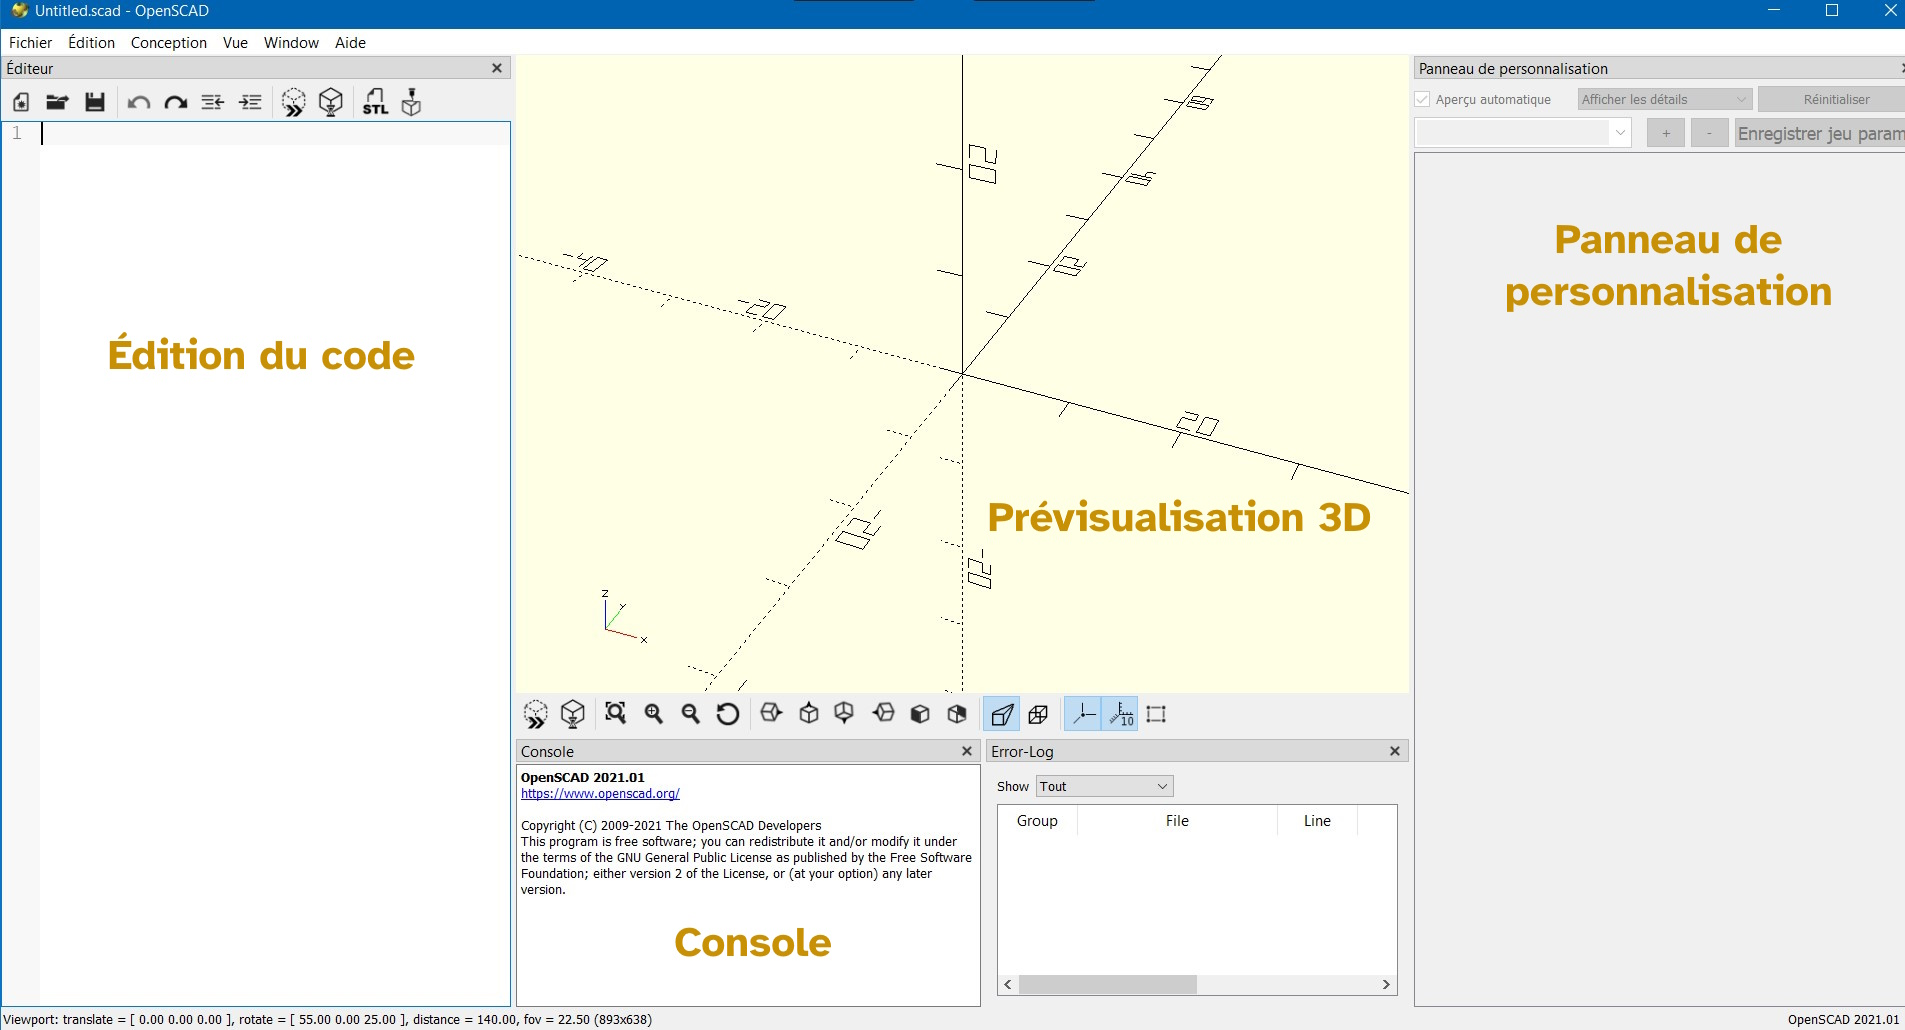
\includegraphics[width=12cm]{images/interface}
	\caption{\textit{Interface d'OpenSCAD}}
\end{figure}


\subsubsection{Éditeur}

C'est dans cette fenêtre que tout le code doit être écrit.
Le fonctionnement est semblable à n'importe quel éditeur classique, il faut rédiger le programme ligne par ligne, elles mêmes numérotées.
L'éditeur d'OpenSCAD fournit un système d'autocomplétion qui peut s'avérer très utile pour connaître rapidement la syntaxe attendue.


\subsubsection{Prévisualisation 3D}

Cette fenêtre permet de visualiser rapidement le rendu 3D décrit par le code.
Il n'est pas possible d'éditer directement les objets dans cette fenêtre.
Toutefois vous pouvez naviguer et explorer le modèle sous tous ses angles, afin de vérifier que le rendu correspond à vos attentes.

Vous pouvez modifier le thème de cette fenêtre en allant dans \textit{édition > préférences > vue 3D}.

Il est également possible de sélectionner les éléments que vous souhaitez voir dans la barre de boutons située au pied de la fenêtre.
Dans cette même barre, des boutons vous permettent de positionner la vue selon des orientations particulières (par exemple parfaitement au dessus du modèle).


\subsubsection{Console}

La console affiche les différentes informations lors de la compilation, le processus de transformation du code vers le modèle 3D.
Elle permet de voir les potentiels avertissements ou erreurs afin de les corriger.


\subsubsection{Panneau de personnalisation}

Nous n'utiliserons pas cette fenêtre dans cet atelier, elle est destinée à des utilisateurs avancés.


\subsection{Premiers pas}

\subsubsection{Formes basiques}

OpenSCAD dispose de plusieurs objets simples pour entamer la création de modèles : 
\verb|square|, \verb|circle|, \verb|cube|, \verb|cylinder| et \verb|sphere|.

Créons par exemple un cube d'1cm de côté. Pour cela il suffit d'écrire \verb|cube(1);| dans l'éditeur.
Ensuite, il faut appuyer sur la touche \verb|F5| de votre clavier pour pouvoir calculer l'aperçu.

\begin{figure}[ht]
	\centering
	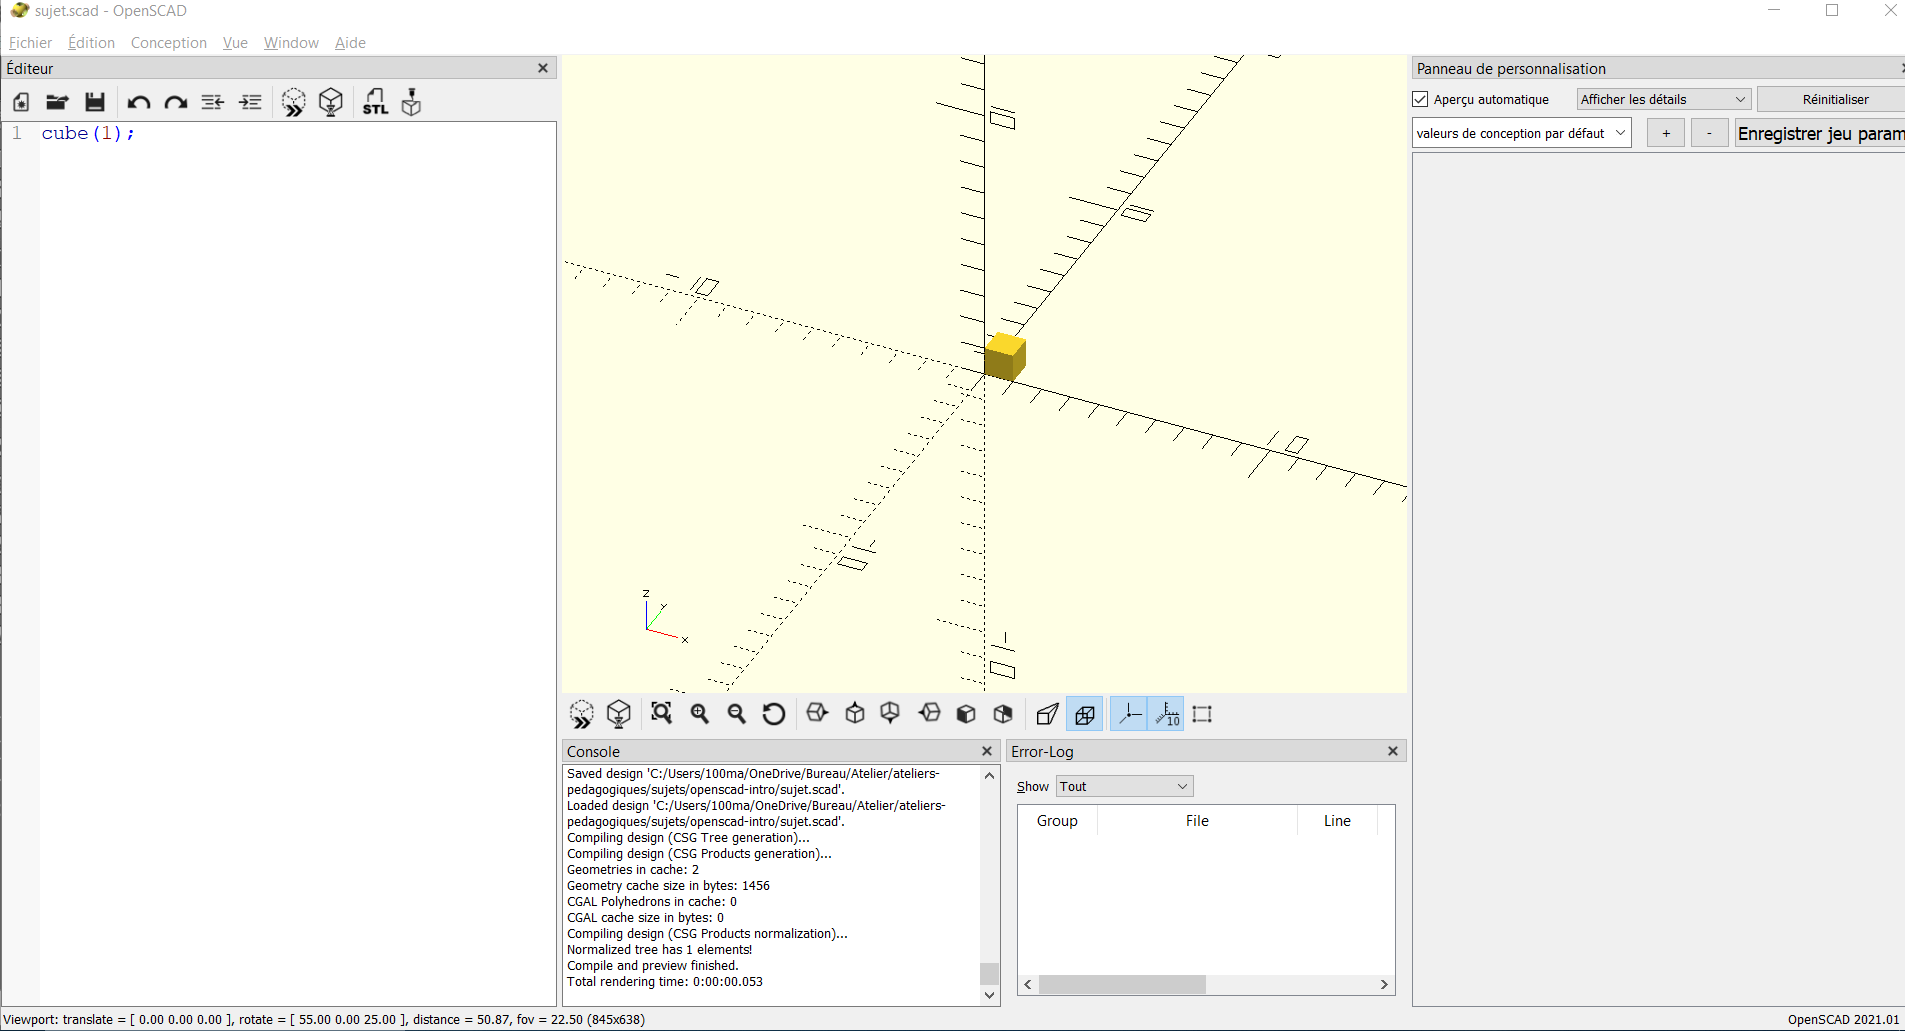
\includegraphics[width=12cm]{images/cube_1}
	\caption{\textit{Simple cube d'1cm de côté}}
\end{figure}

Rajoutons maintenant un pavé droit de 2cm de long, 2cm de large et 0.5cm de haut.
Cela se fait également avec la \textbf{fonction} \verb|cube| mais cette fois en mettant une liste de valeurs en \textbf{paramètre} : \verb|cube([2,2,0.5]);|.

\begin{figure}[ht]
	\centering
	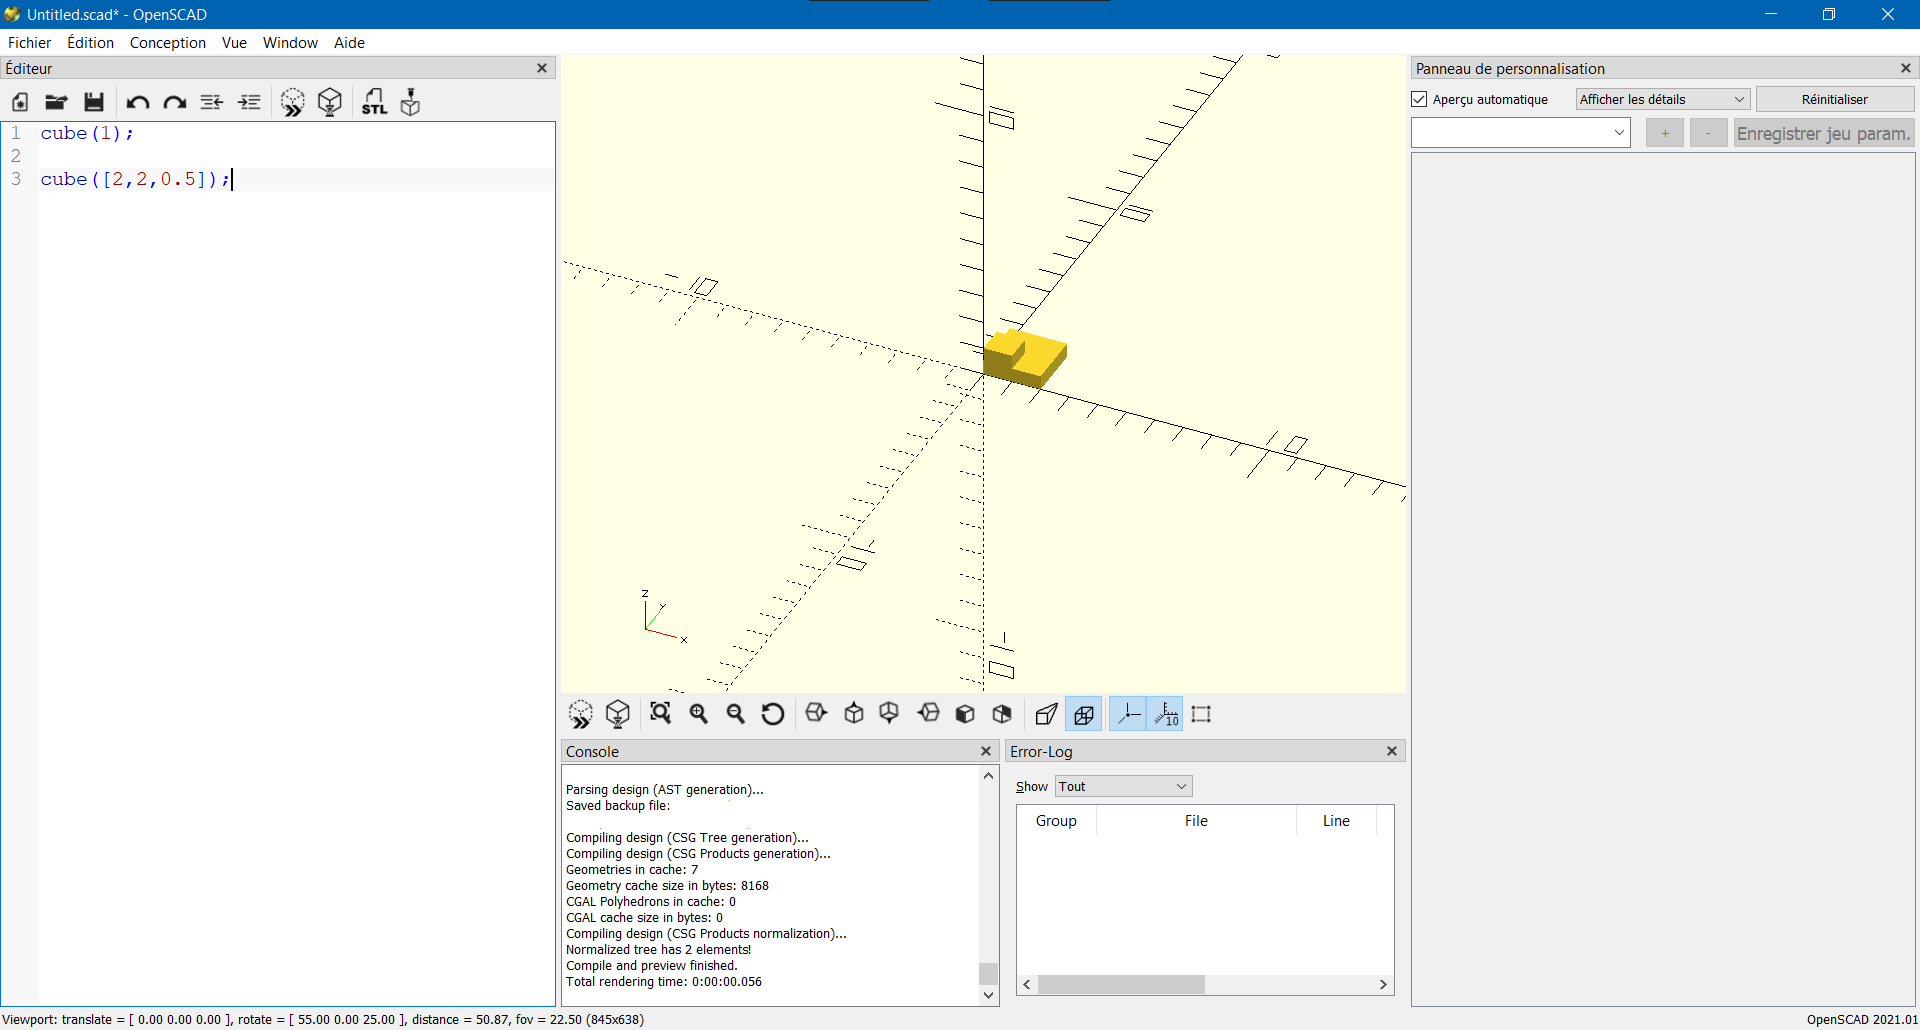
\includegraphics[width=12cm]{images/cube_2-2-05}
	\caption{\textit{Cube et Pavé droit}}
\end{figure}

\hint{
L'ordre des instructions est important. 
Ici, les dimensions sont notées selon l'axe x, puis l'axe y et enfin l'axe z.

Un repère est placé en bas à gauche de la fenêtre de visualisation.}

\warning{
Le langage d'OpenSCAD n'est pas \textit{indent sensitive}, c'est à dire que l'indentation (retours à la ligne et tabulations) ne change en rien l'exécution du programme.
Ainsi, afin de séparer les différents blocs d'instructions, il est nécessaire de mettre un \textbf{;} à la fin.
Sans ces points-virgules, le programme ne pourra pas compiler.}


\subsubsection{Transformations : translations}

Pour le moment, les objets que nous créons sont tous positionnés au même endroit dans l'espace, à partir de l'origine du repère.
Pour pouvoir les déplacer, nous allons appeler la fonction \verb|translate()|.

La syntaxe est la même que pour la création des objets, on indique les valeurs de translation dans une liste (entre crochets) dans l'ordre des axes.

\vspace{12pt}

\begin{figure}[ht]
	\centering
	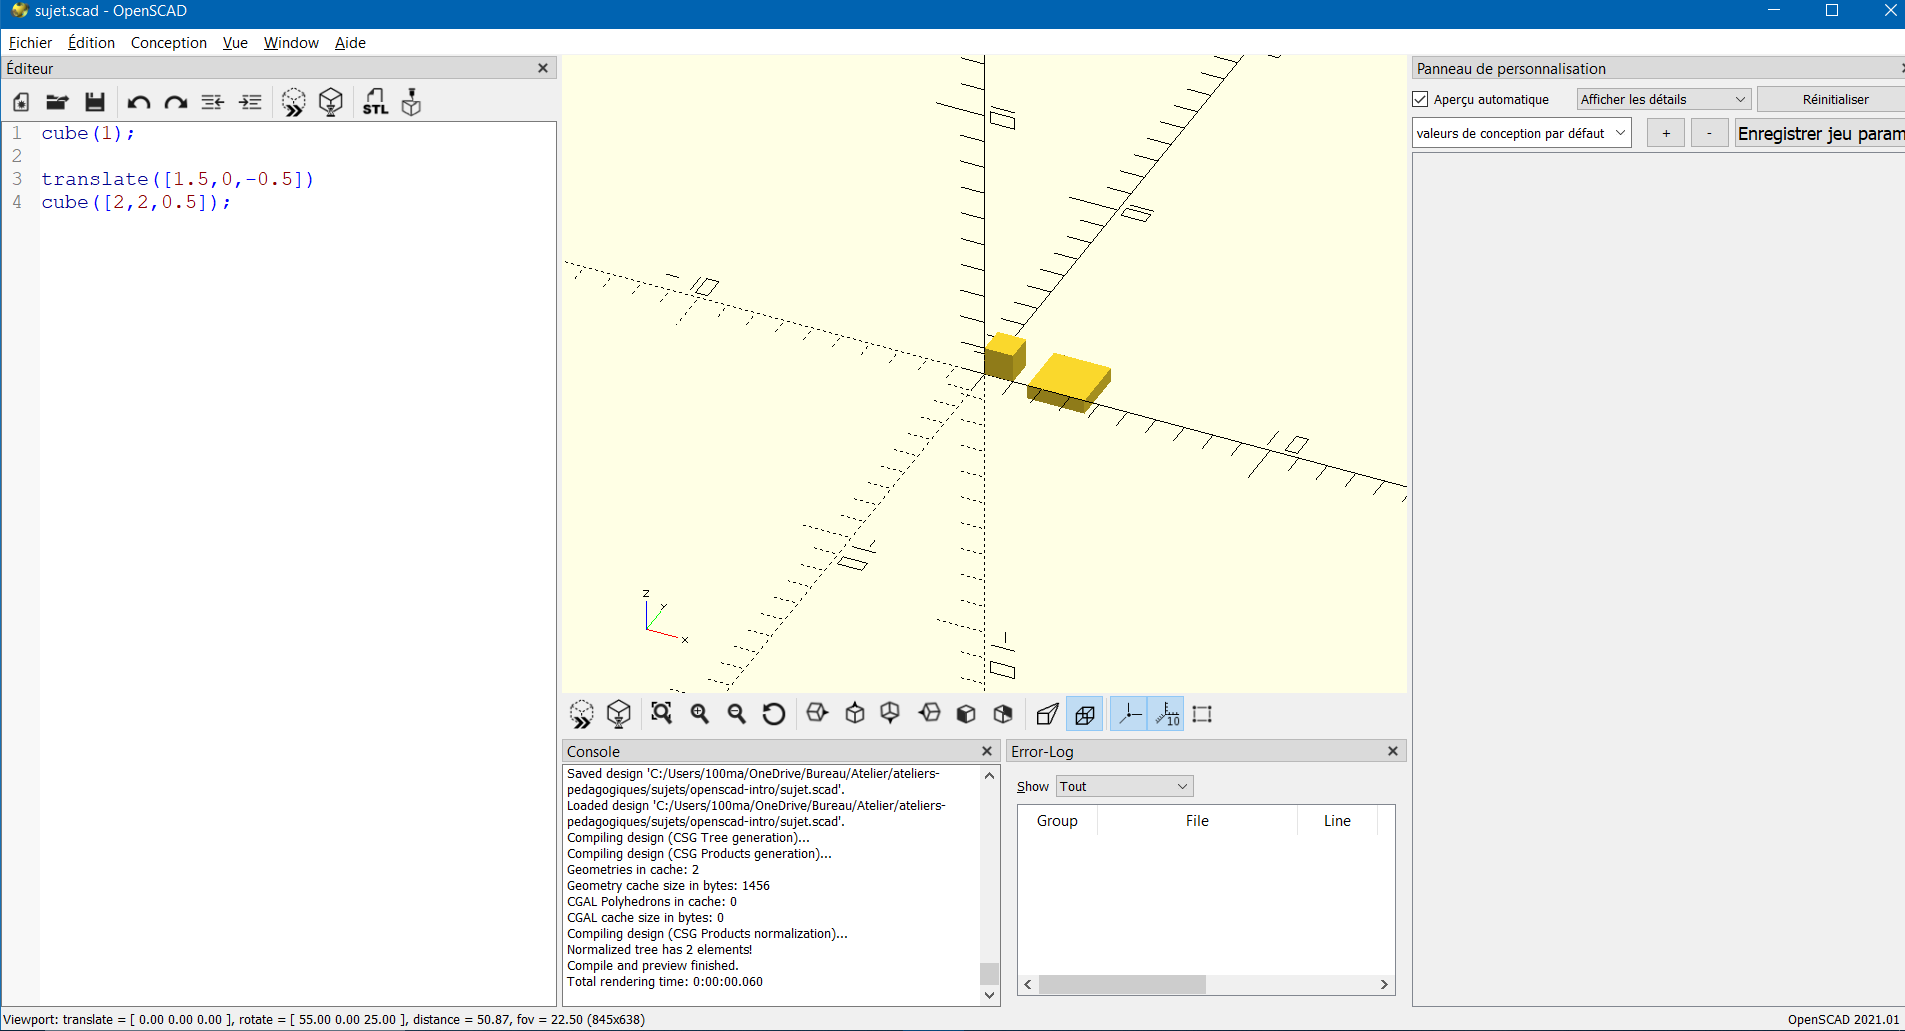
\includegraphics[width=12cm]{images/translate}
	\caption{\textit{Translation du pavé droit}}
\end{figure}

L'exemple suivant crée un cube d'1cm de côté, puis un pavé droit qui est translaté de 1.5 selon l'axe X et -0.5 selon l'axe Z.

La translation n'est appliquée qu'au deuxième objet car un point virgule a été mis après le premier cube.


\subsubsection{Transformations : rotations}

Nous avons comment effectuer des translations, passons désormais aux rotations.
Le fonctionnement est très similaire, il faut utiliser la fonction \verb|rotate()|.

\vspace{12pt}

\begin{figure}[ht]
	\centering
	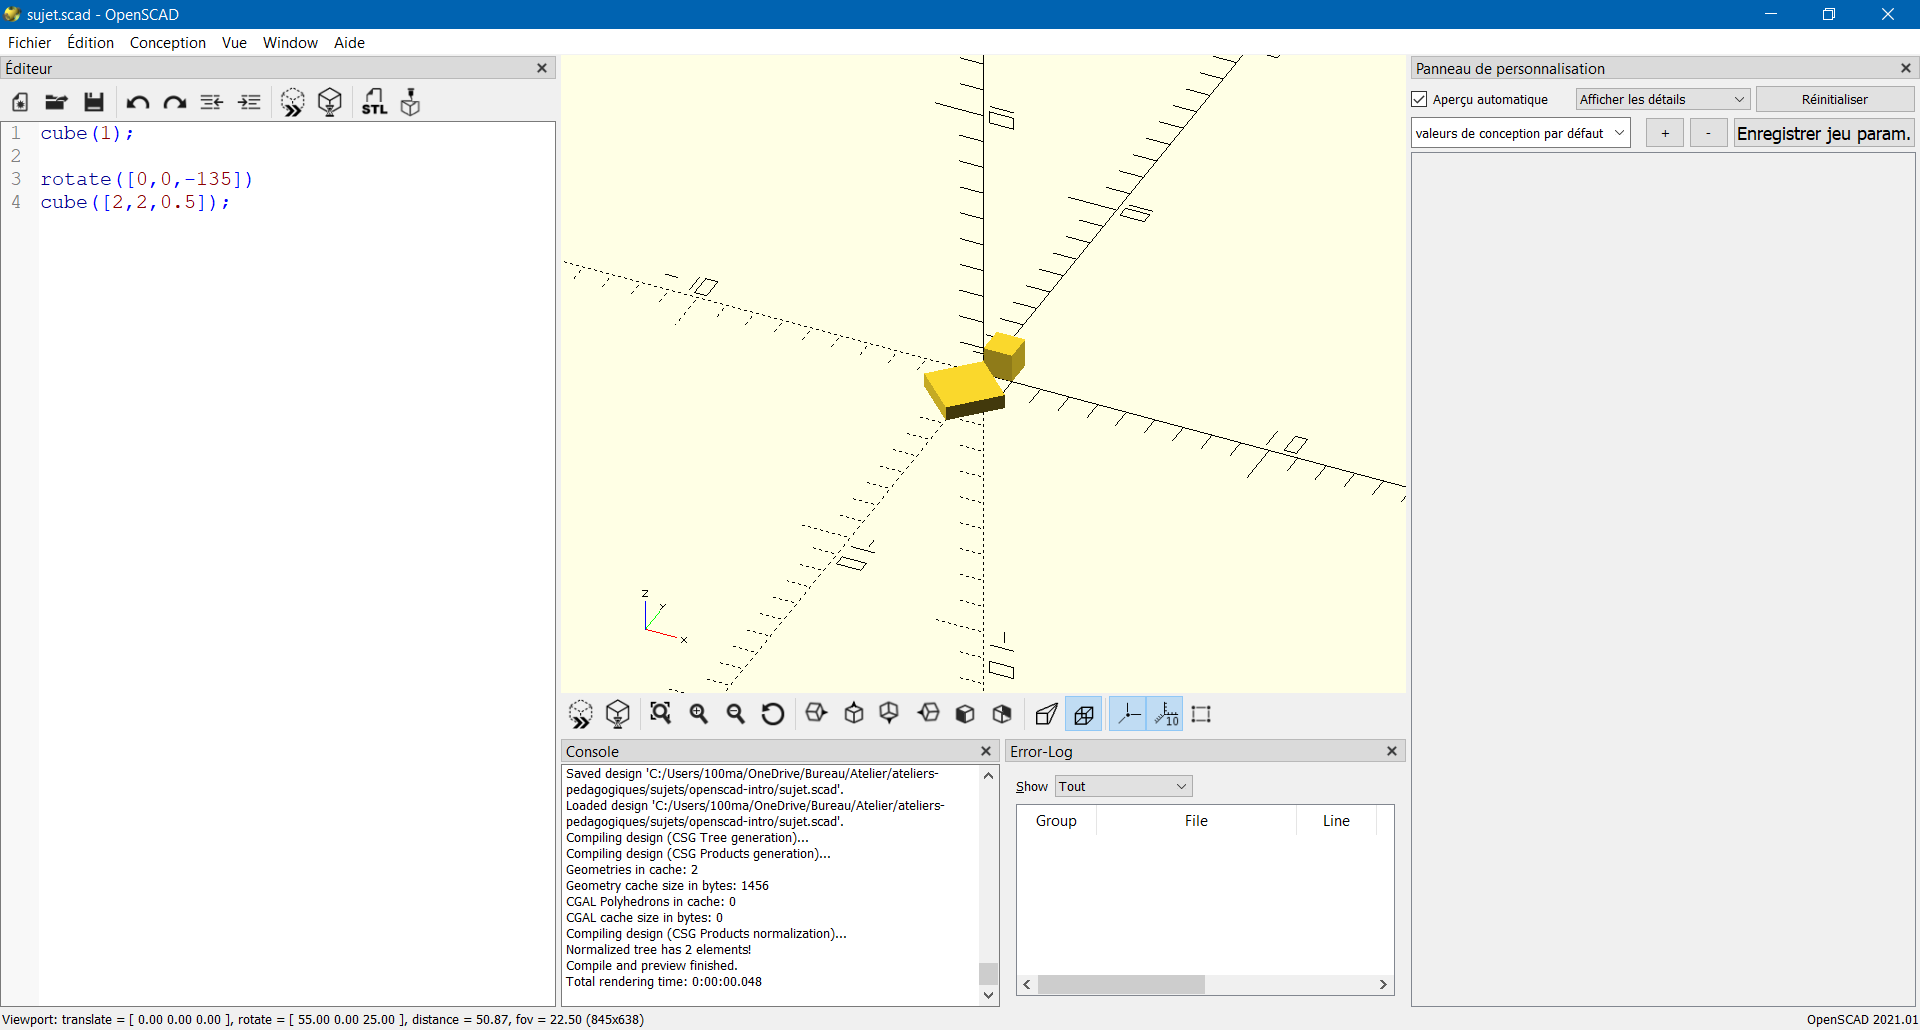
\includegraphics[width=12cm]{images/rotate}
	\caption{\textit{Rotation du pavé droit}}
\end{figure}

L'exemple suivant crée un cube d'1cm de côté, puis un pavé droit auquel est appliquée une rotation de -135° selon l'axe Z (vertical).


\subsubsection{Combinaison d'instructions}

Très souvent — voire quasiment tout le temps — il est nécessaire d'appliquer plusieurs modifications à un même objet. 
Pour cela, il suffit d'écrire les instructions les unes à la suite des autres.

Reprenons par exemple le même modèle (le cube et le pavé) et appliquons une rotation au pavé puis une translation.

\begin{figure}[ht]
	\centering
	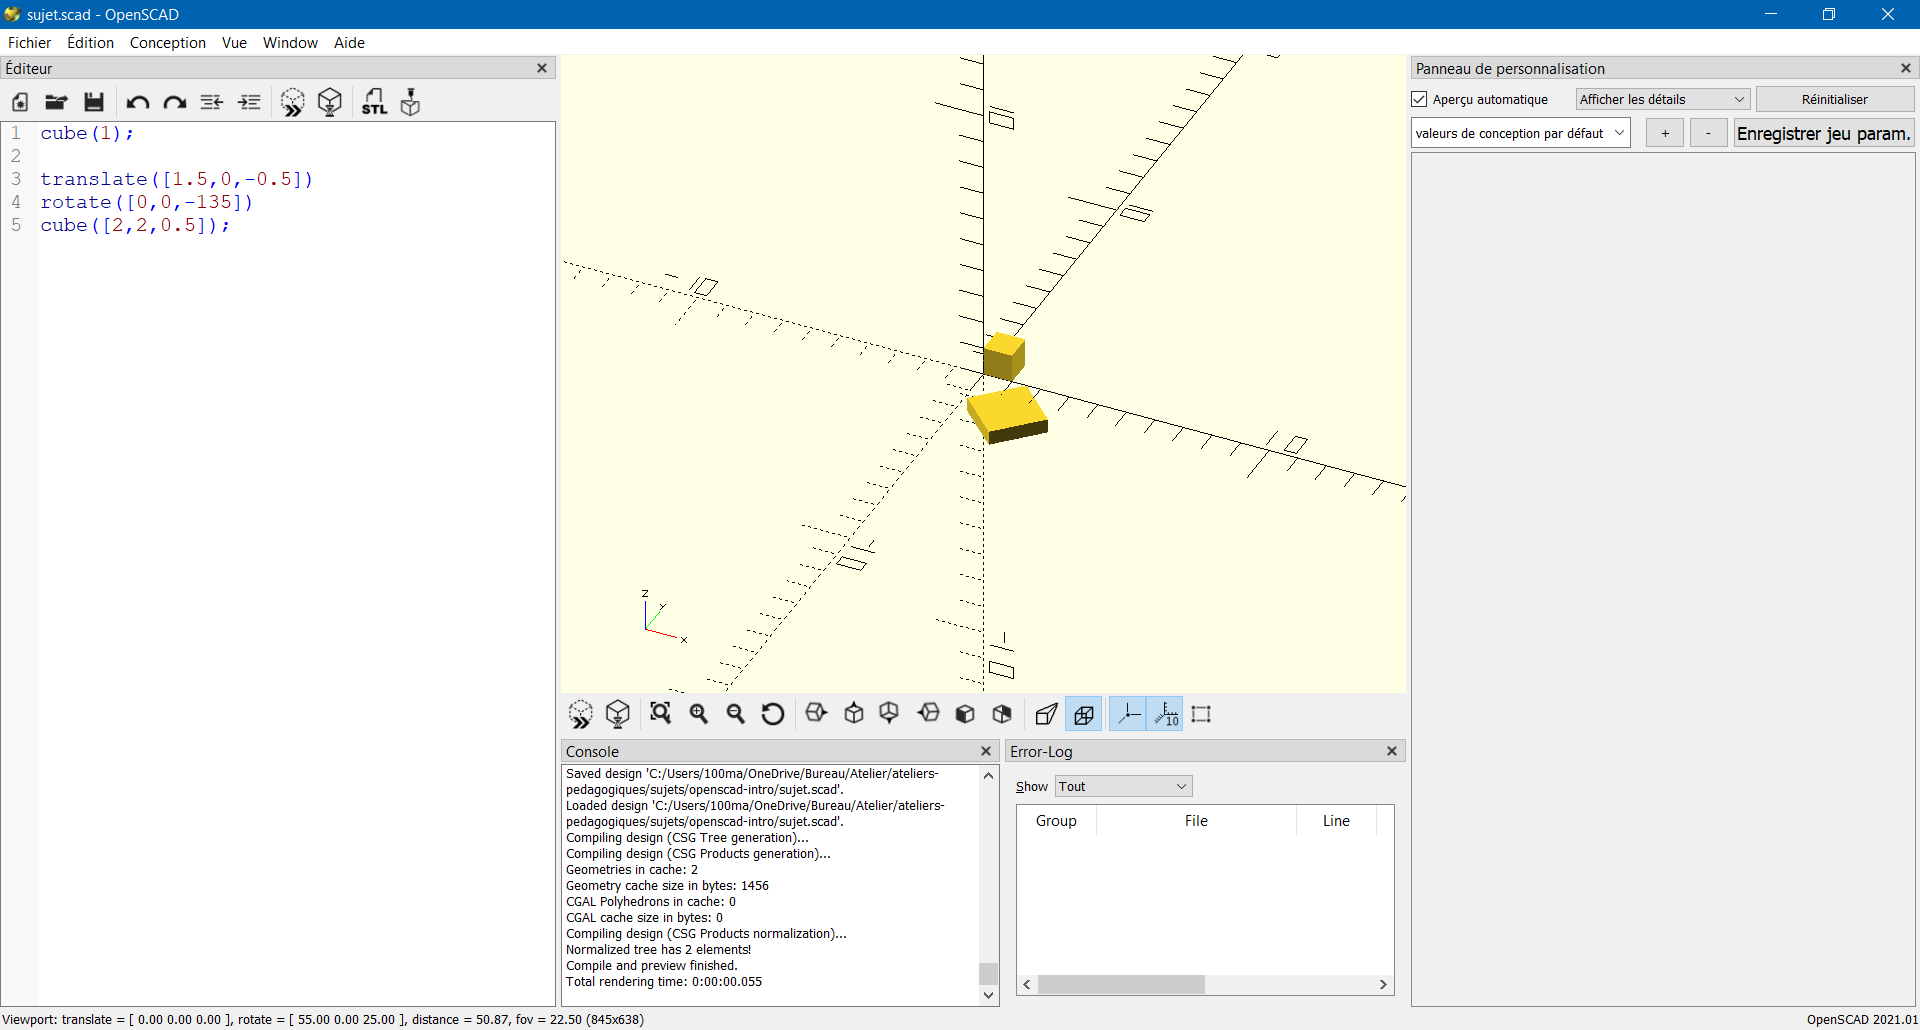
\includegraphics[width=12cm]{images/rotate-translate}
	\caption{\textit{Rotation puis translation du pavé droit}}
\end{figure}

\begin{figure}[ht]
	\centering
	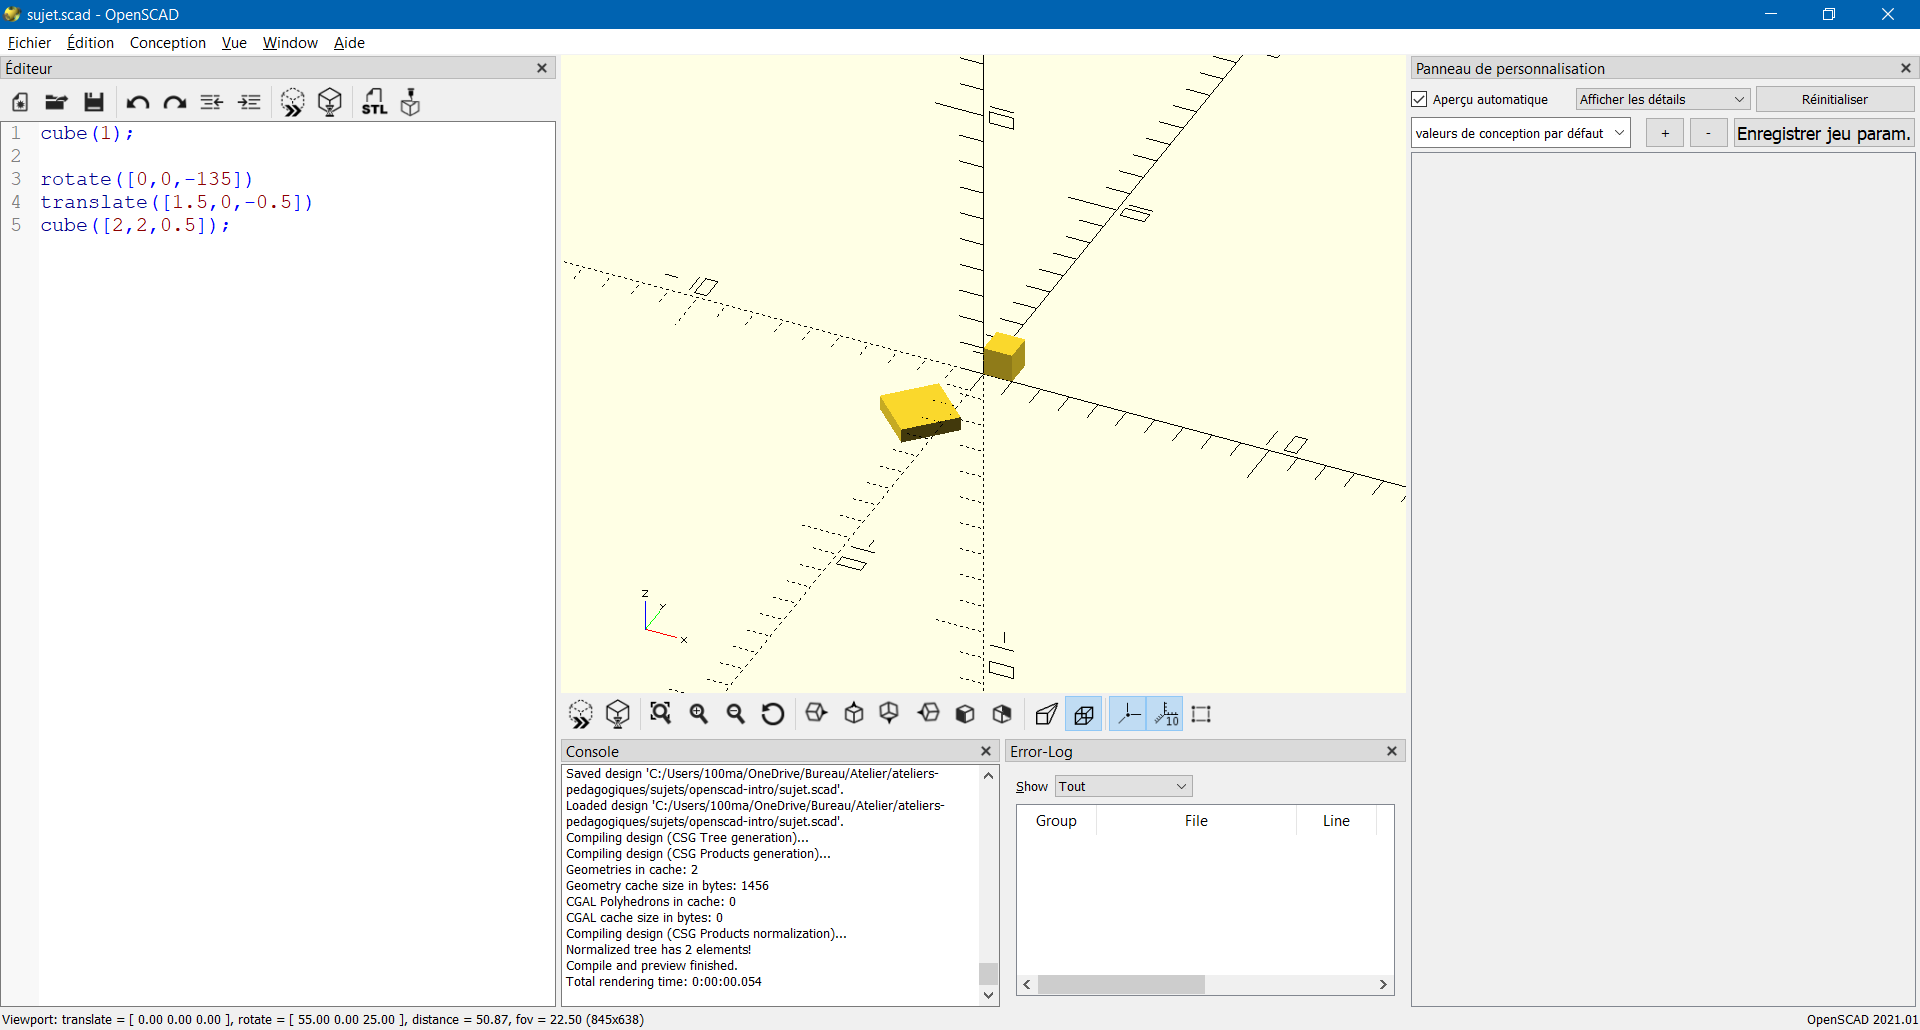
\includegraphics[width=12cm]{images/translate-rotate}
	\caption{\textit{Translation puis rotation du pavé droit}}
\end{figure}

\warning{
L'ordre des instructions est très important.
Il faut lire le code en le "remontant", c'est à dire en partant de la fin du bloc (souvent le modèle de base avec le point-virgule) puis en lisant à l'envers les instructions.

En effet, chaque nouvelle modification s'effectue sur le résultat de la précédente et non sur le modèle à l'origine.}



\subsection{A toi de jouer !}

\subsubsection{Autres instructions}

Vous avez pu voir quelques instructions basiques dans les pages précédentes mais il en existe des dizaines d'autres.
Mais pas de panique, elles sont très faciles à prendre en main, la structure est toujours sensiblement la même.

Le secret pour réaliser votre modèle 3D le plus facilement est de \textbf{lire la documentation}.
Bien évidemment, il ne faut pas faire ça d'un seul coup mais plutôt s'en servir comme un outil d'information, de la même manière qu'un dictionnaire par exemple.

Vous pouvez retrouver en annexe un lien vers un document très important : la \textbf{cheatsheet} d'OpenSCAD.
Cette cheatsheet (feuille de triche) est une page regroupant l'essentiel des informations nécessaires.
En l'occurrence, il y a un lien vers la documentation détaillée de chaque instruction cliquez dessus pour connaitre les détails.

\hint{Si vous avez besoin d'aide, n'hésitez surtout pas à appeler un/e staff qui saura vous guider, ils/elles sont là pour ça !}

\vspace{12pt}
Voici quelques exemples d'instructions qui pourraient vous être utiles :
\begin{itemize}
	\item \verb|scale()| permet de modifier la taille de l'objet.
	\item \verb|color()| permet de colorier l'objet.
	\item \verb|difference() {objet1; objet2; ...}| extrude l'objet2 à l'objet1.
	\item \verb|intersection() {objet1; objet2; ...}| ne conserve que la matière commune à tous les objets.
	\item \verb|text()| crée une surface (2D) selon le texte écrit.
\end{itemize}


\subsubsection{Et maintenant ?}

C'est votre moment!
Vous avez toutes les clés en main pour créer votre propre modèle 3D.
Et en parlant de clés, vous pouvez commencer par créer votre propre \textbf{porte-clés} par exemple.

\hint{Pour cela vous pourriez avoir besoin de créer une forme de base, d'y extruder un trou pour pouvoir passer l'anneau, voir de rajouter votre propre texte.}

\newpage
\section{Annexes}

\subsection{Corrigé des exercices d'application}

\illustrate{exo_1.png}{Envie de buzzer...}

\illustrate{exo_2.png}{Que la lumière soit !}

\illustrate{exo_3.png}{Bientôt DJ ?}

\begin{tcolorbox}[colback=yellow-atelier!10, colframe=gray!70!black, coltitle=black, colbacktitle=gray!70!white, title={\textit{Envie de buzzer...}}, leftrule=2mm]
\begin{small}
\begin{verbatim}
const int button = 1, piezo = 3;

bool is_pressed = false;

void setup(){
  pinMode(button, INPUT);
  pinMode(piezo, OUTPUT);
}

void loop(){  
  if (!is_pressed && digitalRead(button) == HIGH){
    is_pressed = true;
  	analogWrite(piezo, 20); 	// doit être >0 et <1024
  }
  else if (is_pressed && digitalRead(button) == LOW){
    is_pressed = false;
  	analogWrite(piezo, 0);
  }
  
  delay(10);
}
\end{verbatim}
\end{small}
\end{tcolorbox}

\begin{tcolorbox}[colback=yellow-atelier!10, colframe=gray!70!black, coltitle=black, colbacktitle=gray!70!white, title={\textit{Que la lumière soit !}}, leftrule=2mm]
\begin{small}
\begin{verbatim}
const int button = 1, piezo = 3, led_g = 12, led_r = 13;

bool is_pressed = false;

void setup(){
  pinMode(button, INPUT);
  pinMode(piezo, OUTPUT);
  pinMode(led_g, OUTPUT);
  pinMode(led_r, OUTPUT);
}

void loop(){
  if (!is_pressed && digitalRead(button) == HIGH){
    is_pressed = true;
  	analogWrite(piezo, 20); 	// doit être >0 et <1024
    digitalWrite(led_r, LOW);
    digitalWrite(led_g, HIGH);
  }
  else if (is_pressed && digitalRead(button) == LOW){
    is_pressed = false;
  	analogWrite(piezo, 0);
    digitalWrite(led_g, LOW);
    digitalWrite(led_r, HIGH);
  }
  
  delay(10);
}
\end{verbatim}
\end{small}
\end{tcolorbox}

\begin{tcolorbox}[colback=yellow-atelier!10, colframe=gray!70!black, coltitle=black, colbacktitle=gray!70!white, title={\textit{Bientôt DJ ?}}, leftrule=2mm]
\begin{small}
\begin{verbatim}
const int button = 1, piezo = 3, led_g = 12, led_r = 13, potentiometer = A0;

bool is_pressed = false;
int frequency = 0;

void setup(){
  pinMode(button, INPUT);
  pinMode(piezo, OUTPUT);
  pinMode(led_g, OUTPUT);
  pinMode(led_r, OUTPUT);
}

void loop(){
  frequency = analogRead(potentiometer) *20 / 1023;
  
  if (!is_pressed && digitalRead(button) == HIGH){
    is_pressed = true;
  	analogWrite(piezo, frequency);
    digitalWrite(led_r, LOW);
    digitalWrite(led_g, HIGH);
  }
  else if (is_pressed && digitalRead(button) == LOW){
    is_pressed = false;
  	analogWrite(piezo, 0);
    digitalWrite(led_g, LOW);
    digitalWrite(led_r, HIGH);
  }
  
  delay(10);
}
\end{verbatim}
\end{small}
\end{tcolorbox}

\clearpage
\subsection{Liens utiles}

\begin{itemize}
	\item \doclink{https://www.tinkercad.com}{Tinkercad}
	\item \doclink{https://docs.arduino.cc/}{Documentation Arduino}
	\item \doclink{https://www.electronics-tutorials.ws/}{Pour aller plus loin}
		  Ce site contient divers cours d'électronique très détaillés et facilement compréhensibles.
		  N'hésitez pas à y jeter un oeil pour comprendre plus en détail les concepts et composants abordés.
\end{itemize}


\end{document}
